\documentclass[12pt, a4paper]{article}

% Imports
\usepackage{times}
\usepackage{array}
\usepackage[T1]{fontenc}
\usepackage{lmodern}
\usepackage{parskip}
\usepackage[hidelinks, pdfusetitle]{hyperref}
\usepackage{url}
\usepackage{titling}
\usepackage{fancyhdr}
\usepackage{titlefoot}
\usepackage{booktabs}
\usepackage{enumitem}
\usepackage{csquotes}
\usepackage{multicol}
\usepackage{tikz}
\usetikzlibrary{arrows,shapes}
\usetikzlibrary{positioning, arrows.meta, shapes.geometric}
\usepackage{tikz}
\usepackage{graphicx}
\usepackage{tabularx}
\usepackage{lmodern}
\usepackage{array}
\usepackage{ragged2e}
\usepackage{amsmath}
\usepackage{bm}
\usepackage{lmodern}
\usepackage{ltablex}  % Combina le funzionalità di tabularx con longtable
\keepXColumns        % Mantiene il comportamento della colonna "X"
\usepackage{longtable}
\usepackage{amsthm}
\usepackage{amssymb}
\usepackage{tikz-cd}
\usepackage{geometry}
 \geometry{
 a4paper,
 total={170mm,257mm},
 left=20mm,
 top=20mm,
 }
% Rules
\setlength{\headheight}{16pt}
\pagestyle{fancy}
\let\orighref\href
\frenchspacing
\makeatletter
\def\thm@space@setup{%
  \thm@preskip=\parskip \thm@postskip=0pt
}
\makeatother

% Env
\newtheorem{theorem}{Theorem}[section]
\newtheorem*{bigtheorem}{Theorem}
\newtheorem{lemma}[theorem]{Lemma}
\newtheorem{corollary}[theorem]{Corollary}
\theoremstyle{definition}
\newtheorem{definition}[theorem]{Definition}
\newtheorem{proposition}[theorem]{Proposition}
\newtheorem{example}[theorem]{Example}
\newtheorem{conjecture}[theorem]{Conjecture}

% Commands
\renewcommand{\href}[2]{\orighref{#1}{#2\ \faExternalLink}}
\newcommand{\Conjugate}[1]{\overline{ #1 }}
\newcommand{\Complex}{\mathbb{C}}
\newcommand{\ComplexNumbers}{\mathbb{C}}
\newcommand{\Integers}{\mathbb{Z}}
\newcommand{\ImaginaryPart}{\operatorname{Im}}
\newcommand{\ImaginaryNumbers}{\mathbb{I}}
\newcommand{\NaturalNumbers}{\mathbb{N}}
\newcommand{\Quaterions}{\mathbb{H}}
\newcommand{\Rational}{\mathbb{Q}}
\newcommand{\RationalNumbers}{\mathbb{Q}}
\newcommand{\Real}{\mathbb{R}}
\newcommand{\RealNumbers}{\mathbb{R}}
\newcommand{\RealPart}{\operatorname{Re}}
\newcommand{\AutomorphismGroup}{\operatorname{Aut}}
\newcommand{\Automorphisms}{\operatorname{Aut}}
\newcommand{\Codimension}{\operatorname{codim}}
\newcommand{\GeneralLinear}{\operatorname{GL}}
\newcommand{\Homomorphisms}{\operatorname{Hom}}
\newcommand{\HomomorphismGroup}{\operatorname{Hom}}
\newcommand{\InnerProduct}[2]{\langle #1 , #2 \rangle}
\newcommand{\InnerProductLabeled}[3]{{\langle #1 , #2 \rangle}_{ #3 }}
\newcommand{\Identity}{\mathrm{Id}}
\newcommand{\Image}{\operatorname{Im}}
\newcommand{\Kernel}{\ker}
\newcommand{\ProjectiveSpace}{\mathbb{P}}
\newcommand{\Projective}{\mathbb{P}}
\newcommand{\Range}{\operatorname{Range}}
\newcommand{\Trace}{\operatorname{Tr}}
\newcommand{\Transpose}[1]{{ #1 }^T}
\renewcommand{\tabularxcolumn}[1]{>{\RaggedRight\arraybackslash}m{#1}}
\renewcommand{\arraystretch}{1.2} % Spaziatura verticale nelle righe



\title{\texorpdfstring{%
    
\includegraphics[scale=0.3]{./public/unina-logo.jpg}\\ \vspace{0.5cm}%
    Corso di Laurea in Ingegneria Informatica\\%
    \vspace{0.5cm}
    Corso di Ingegneria Del Software\\%
    Prof. \textbf{Roberto Pietrantuono}\\%
    a.a. 2024-2025 \\
    \vspace{0.5cm}
    Progetto \\
    \textbf{Comics Store}
}{Corso di Laurea in Ingegneria Informatica}}

\author{\textbf{Autori}\\ \textbf{Alessio Romano} N46007394 alessio.romano02dev@gmail.com \\ \textbf{Mattia Gifuni} N46007229 mat.gifuni@studenti.unina.it}

\begin{document}
\maketitle

\newpage
\tableofcontents
\newpage

\section{Specifiche Informali}
Si vuole realizzare un sistema software per la gestione di una fumetteria.

Il sistema consente la vendita dei fumetti in negozio, il ritiro in negozio, e la consegna a domicilio.

Per ogni fumetto è specificato il nome della serie (es.: “Diabolik”), l’anno della serie (es: “LXII”, oppure “2010”), il numero del volume, il titolo, il genere (Supereroi, Azione, Fantasy, Manga, …), la casa editrice, una immagine di copertina, una eventuale descrizione e il prezzo. La fumetteria tiene traccia del numero di copie che ha a disposizione per ogni articolo.

Il titolare del negozio si occupa dell’inserimento dei commessi nel sistema, specificando nome, cognome, username e password.

I commessi si occupano della vendita degli articoli presso il punto vendita, accedendo al sistema con le proprie credenziali. Per ogni nuovo arrivo, un commesso acquisisce in negozio l’immagine di copertina con un apposito scanner, inserisce manualmente i dati del fumetto. Gli impiegati devono anche poter modificare il numero di copie a disposizione di un fumetto, all’atto di una vendita in negozio.

I clienti online hanno la possibilità di consultare la vetrina web ed acquistare gli articoli accedendo all’applicazione web della fumetteria, per poi ritirare l’acquisto in negozio, ovvero richiederne la consegna a domicilio. Un cliente online può visualizzare la lista dei prodotti disponibili effettuando ricerche per genere o per serie.

I clienti hanno la possibilità di registrarsi accedendo a promozioni speciali o per ricevere la newsletter con le novità in arrivo. Per registrarsi devono fornire nome, cognome, username, password, e-mail e indirizzo.

Il cliente effettua l’acquisto con carta di credito, selezionando i fumetti dopo una ricerca. I clienti registrati ottengono il 10% di sconto per ogni acquisto e possono richiedere la consegna a domicilio, con un modico costo supplementare che viene sommato al totale dell’ordine immediatamente prima del pagamento.

Prima di accettare un ordine, il sistema controlla l’effettiva disponibilità degli articoli richiesti, ed in caso positivo, al termine del pagamento, invia la conferma per e-mail al cliente.

In caso di ritiro in negozio, la mail di conferma contiene un codice QR (se non registrato, il cliente deve fornire un indirizzo e-mail all’atto dell’acquisto). Al ritiro in negozio, il cliente presenta il codice QR e il commesso lo legge con un apposito lettore, in modo che la vendita risulti completata (il sistema registra la data di ritiro).

Per ogni acquisto online il sistema notifica ai commessi la ricezione del nuovo ordine, contenente la lista dei fumetti acquistati. Per ogni vendita online di cui il cliente abbia richiesto la consegna a domicilio, un commesso predispone il pacco per la consegna e tramite il sistema richiede ad una società di riders il ritiro in negozio e la consegna al cliente. Effettuata la consegna, il sistema dello spedizioniere comunica automaticamente al sistema della fumetteria l’avvenuta consegna dell’ordine. Per una vendita online, il numero delle copie a disposizione viene automaticamente decrementato all’atto dell’acquisto (indipendentemente dalla modalità di ritiro).

Il titolare del negozio predispone una newsletter con i nuovi arrivi, o per comunicare eventi come lapartecipazione a fiere di settore, o per promozioni con sconti speciali, che il sistema invia mensilmente per e-mail ai clienti registrati.

\newpage

\section{Analisi e specifica dei requisiti}
\subsection{Revisione dei requisiti}

\begin{enumerate}

\item Il sistema deve memorizzare per ogni fumetto i seguenti dati:
  \begin{enumerate}
    \item Nome della serie (es. “Diabolik”).
    \item Anno della serie (in formato romano, es. “LXII”, oppure in formato arabo, es. “2010”).
    \item Numero del volume.
    \item Titolo.
    \item Genere (es. Supereroi, Azione, Fantasy, Manga, …).
    \item Casa editrice.
    \item Immagine di copertina.
    \item Eventuale descrizione.
    \item Prezzo.
  \end{enumerate}

\item Il sistema deve tenere traccia del numero di copie a disposizione per ciascun fumetto.

\item Il sistema deve permettere al titolare del negozio di inserire i dati relativi ai commessi.

\item Per ogni commesso il sistema deve memorizzare:
  \begin{enumerate}
    \item Nome.
    \item Cognome.
    \item Username.
    \item Password.
  \end{enumerate}

\item Il sistema deve consentire ai commessi di autenticarsi utilizzando le proprie credenziali.

\item Il sistema deve abilitare i commessi ad acquisire, per ogni nuovo arrivo, l’immagine di copertina di un fumetto mediante uno scanner.

\item Il sistema deve consentire ai commessi di inserire manualmente i dati dei fumetti.

\item Il sistema deve permettere agli impiegati di modificare il numero di copie disponibili di un fumetto in seguito a una vendita in negozio.

\item Il sistema deve supportare la vendita dei fumetti direttamente in negozio, aggiornando il numero delle copie al momento della vendita.

\item Il sistema deve offrire una vetrina web che consenta ai clienti online di consultare l’elenco dei fumetti disponibili.

\item Il sistema deve permettere ai clienti online di effettuare ricerche dei fumetti per genere o per serie.

\item Il sistema deve consentire ai clienti online di selezionare i fumetti e procedere all’acquisto mediante carta di credito.

\item Prima di confermare un ordine online, il sistema deve verificare l’effettiva disponibilità degli articoli selezionati.

\item Al termine del pagamento, se la disponibilità è confermata, il sistema deve inviare al cliente una mail di conferma d’ordine.

\item Il sistema deve notificare ai commessi la ricezione di ogni nuovo ordine online, specificando l’elenco dei fumetti acquistati.

\item Per ogni vendita online, il sistema deve decrementare automaticamente il numero delle copie disponibili dei fumetti acquistati, indipendentemente dalla modalità di ritiro scelta.

\item Il sistema deve consentire al cliente online di scegliere tra due modalità di ricezione dell’ordine: ritiro in negozio oppure consegna a domicilio.

\item In caso di ritiro in negozio:
  \begin{enumerate}
    \item Il sistema deve inviare una mail di conferma contenente un codice QR al cliente registrato.
    \item Se il cliente non è registrato, il sistema deve richiedere l’indirizzo e-mail al momento dell’acquisto per poi inviare il codice QR.
    \item Al ritiro in negozio, il sistema deve permettere al commesso, tramite un apposito lettore, di verificare il codice QR presentato dal cliente e registrare la data di ritiro.
  \end{enumerate}

\item In caso di consegna a domicilio:
  \begin{enumerate}
    \item Un commesso deve poter predisporre il pacco per la consegna.
    \item Il sistema deve permettere al commesso di inviare una richiesta a una società di riders per il ritiro in negozio e la consegna al cliente.
    \item Il sistema deve ricevere automaticamente una conferma dallo spedizioniere al momento dell’avvenuta consegna.
  \end{enumerate}

\item Il sistema deve consentire ai clienti di registrarsi fornendo: nome, cognome, username, password, e-mail e indirizzo.

\item Il sistema deve consentire ai clienti registrati di accedere all’applicazione web della fumetteria.

\item Il sistema deve applicare uno sconto del 10\% sull’acquisto dei fumetti per i clienti registrati.

\item Il sistema deve permettere al titolare del negozio di predisporre una newsletter contenente:
  \begin{enumerate}
    \item I nuovi arrivi.
    \item Comunicazioni su eventi (es.\ partecipazioni a fiere di settore).
    \item Promozioni con sconti speciali.
  \end{enumerate}

\item Il sistema deve inviare mensilmente per e-mail la newsletter ai clienti registrati.
\end{enumerate}

\newpage

\subsection{Glossario dei Termini}

Di seguito viene riportato un glossario dei termini utilizzati nella revisione dei requisiti

\begin{center}
\begin{tabularx}{0.95\textwidth}{|X|X|X|}
\hline
\textbf{Termine} & \textbf{Descrizione} & \textbf{Sinonimi} \\
\hline
\textbf{Commessi} & Lo staff che si occupa della gestione e della vendita & Dipendenti / Impiegati \\
\hline
\textbf{Clienti Online} & Qualunque utente, registrato e non, che visita il negozio online & N/A \\
\hline
\textbf{Clienti Registrati} & Qualunque cliente, con un account utente registrato sullo store online & N/A \\
\hline
\textbf{Clienti non Registrati} & Qualunque cliente, senza un account utente registrato sul negozio online & Guest \\
\hline
\textbf{Spedizioniere} & Servizio di spedizione di terze parti & Società di Riders \\
\hline
\textbf{Vendita Online} & Qualunque vendita effettuata sul negozio online, a prescindere dalla registrazione dell'utente e dal metodo di consegna & N/A \\
\hline
\end{tabularx}
\end{center}

\section{Classificazione dei requisiti}
\subsection{Requisiti Funzionali}
Di seguito viene riportata la tabella contenente i requisiti funzionali relativi alla specifica, e la corrispettiva origine dalla revisione dei requisiti.

\begin{longtable}{|
    >{\centering\arraybackslash}m{0.10\textwidth} |   % colonna ID, centrata verticalmente
    >{\raggedright\arraybackslash}m{0.70\textwidth} | % colonna Descrizione, allineata a sinistra
    >{\centering\arraybackslash}m{0.10\textwidth} |   % colonna Origine, centrata verticalmente
}
\hline
\textbf{ID} & \textbf{Descrizione} & \textbf{Origine} \\
\hline
\endfirsthead

\hline
\textbf{ID} & \textbf{Descrizione} & \textbf{Origine} \\
\hline
\endhead

\textbf{RF01} & Il sistema deve memorizzare per ogni fumetto i seguenti dati: nome della serie,  
anno della serie (in formato romano o arabo), numero del volume, titolo, genere, casa editrice,  
immagine di copertina, eventuale descrizione, prezzo e quantità disponibile. & 1,2 \\
\hline
\textbf{RF02} & Il sistema deve permettere al titolare del negozio di inserire i dati relativi ai commessi  
e di memorizzare: nome, cognome, username e password. & 3,4 \\
\hline
\textbf{RF03} & Il sistema deve consentire ai commessi di autenticarsi utilizzando le proprie credenziali,  
deve abilitare i commessi ad acquisire, per ogni nuovo arrivo, l’immagine di copertina di un fumetto  
mediante uno scanner, e deve permettere ai commessi di inserire manualmente i dati dei fumetti. & 5,6 \\
\hline
\textbf{RF04} & Il sistema deve permettere agli impiegati di modificare il numero di copie disponibili di un fumetto  
in seguito a una vendita in negozio e deve supportare la vendita dei fumetti direttamente in negozio,  
aggiornando il numero delle copie al momento della vendita. & 8 \\
\hline
\textbf{RF05} & Il sistema deve offrire una vetrina web che consenta ai clienti online di consultare  
l’elenco dei fumetti disponibili e deve permettere ai clienti online di effettuare ricerche dei fumetti  
per genere o per serie. & 10,11 \\
\hline
\textbf{RF06} & Il sistema deve consentire ai clienti online di selezionare i fumetti e procedere  
all’acquisto mediante carta di credito. & 12 \\
\hline
\textbf{RF07} & Prima di confermare un ordine online, il sistema deve verificare l’effettiva disponibilità  
degli articoli selezionati. & 13 \\
\hline
\textbf{RF08} & Al termine del pagamento, se la disponibilità è confermata, il sistema deve inviare  
al cliente una mail di conferma d’ordine. & 14 \\
\hline
\textbf{RF09} & Il sistema deve notificare ai commessi la ricezione di ogni nuovo ordine online,  
specificando l’elenco dei fumetti acquistati. & 15 \\
\hline
\textbf{RF10} & Per ogni vendita online, il sistema deve decrementare automaticamente il numero delle copie  
disponibili dei fumetti acquistati, indipendentemente dalla modalità di ritiro scelta. & 16 \\
\hline
\textbf{RF11} & Il sistema deve consentire al cliente online di scegliere tra due modalità di ricezione  
dell’ordine: ritiro in negozio oppure consegna a domicilio. & 17 \\
\hline
\textbf{RF12} & (Ritiro in negozio) Il sistema deve inviare una mail di conferma contenente un codice QR  
al cliente registrato; se il cliente non è registrato, il sistema deve richiedere l’indirizzo e-mail  
al momento dell’acquisto per poi inviare il codice QR. & 18(a,b)\\
\hline
\textbf{RF13} & (Ritiro in negozio) Al ritiro, il sistema deve permettere al commesso, tramite un apposito  
lettore, di verificare il codice QR presentato dal cliente e registrare la data di ritiro. & 18(c) \\
\hline
\textbf{RF14} & (Consegna a domicilio) Un commesso deve poter predisporre il pacco per la consegna; il sistema  
deve permettere al commesso di inviare una richiesta a una società di riders per il ritiro in negozio  
e la consegna al cliente; inoltre deve ricevere automaticamente una conferma dallo spedizioniere  
al momento dell’avvenuta consegna. & 19 \\
\hline
\textbf{RF15} & Il sistema deve consentire ai clienti di registrarsi fornendo: nome, cognome, username,  
password, e-mail e indirizzo. & 20\\
\hline
\textbf{RF16} & Il sistema deve consentire ai clienti registrati di accedere all’applicazione web  
della fumetteria, applicando uno sconto del 10\% sull’acquisto dei fumetti per i clienti registrati. & 21,22 \\
\hline
\textbf{RF17} & Il sistema deve permettere al titolare del negozio di predisporre una newsletter contenente:  
nuovi arrivi, comunicazioni su eventi e promozioni con sconti speciali, e deve inviare mensilmente  
per e-mail la newsletter ai clienti registrati. & 23 \\
\hline
\end{longtable}

\subsubsection{Vincoli/Requisiti non funzionali}
Di seguito viene riportata la tabella contenente i vincoli e requisiti non funzionali derivante dalla specifica.
\begin{center}
\begin{tabularx}{1\textwidth}{|>{\hsize=0.13\hsize}X|>{\hsize=0.8\hsize}X|}
\hline
\textbf{ID} & \textbf{Requisito} \\
\hline
\textbf{V/RNF01} & Il sistema deve garantire la sicurezza degli accessi tramite credenziali per i commessi e per i clienti. \\
\hline
\textbf{V/RNF02} & Il sistema deve verificare l’effettiva disponibilità degli articoli prima di accettare un ordine, assicurando l’affidabilità delle transazioni. \\
\hline
\textbf{V/RNF03} & Il sistema deve potersi integrare automaticamente con sistemi esterni, come quello dello spedizioniere. \\
\hline
\textbf{V/RNF04} & L’interfaccia utente deve essere semplice e intuitiva, adatta sia a clienti online che a commessi in negozio. \\
\hline
\textbf{V/RNF05} & Le comunicazioni automatiche come newsletter o conferme devono essere generate e inviate in modo periodico. \\
\hline
\textbf{V/RNF06} & Il numero di copie disponibili di ogni fumetto deve essere aggiornato in tempo reale al momento dell’acquisto. \\
\hline
\textbf{V/RNF07} & L'applicazione web deve essere accessibile tramite diversi dispositivi e browser, garantendo una buona portabilità. \\
\hline
\textbf{V/RNF08} & Il sistema deve strutturare in modo coerente e completo i dati relativi ai fumetti: nome serie, anno serie (formato romano o arabo), numero volume, titolo, genere, casa editrice, immagine copertina, descrizione, prezzo, quantità. \\
\hline
\textbf{V/RNF09} & Il sistema deve strutturare in modo coerente e completo i dati relativi ai commessi: nome, cognome, username, password. \\
\hline
\textbf{V/RNF10} & Il sistema deve strutturare in modo coerente e completo i dati relativi ai clienti registrati: nome, cognome, username, password, e-mail, indirizzo. \\
\hline
\end{tabularx}
\end{center}

\newpage
\subsection{Modellazione dei casi d’uso}
\subsubsection{Attori e casi d’uso}
\textbf{\textit{Attori Primari:}}
\begin{multicols}{2}
  \begin{itemize}
    \item Titolare
    \item Commesso
    \item Cliente Online
    \item Cliente in Negozio
  \end{itemize}
\end{multicols}
% --- Attori Secondari ---
\textbf{\textit{Attori Secondari:}}
\begin{multicols}{2}
  \begin{itemize}
    \item Sistema e-mail
    \item Servizio Riders
    \item Lettore QR
    \item Scanner copertine
  \end{itemize}
\end{multicols}

% --- Casi d’uso ---
\textbf{\textit{Casi d’uso:}}
\begin{itemize}
  \item UC1: Gestisci Anagrafica Fumetto
  \item UC2: Gestisci Scorte Fumetto
  \item UC3: Gestisci Anagrafica Commessi
  \item UC4: Autentica Commesso
  \item UC5: Acquisisci Copertina Fumetto
  \item UC6: Inserisci Dati Fumetto
  \item UC7: Vendi in Negozio
  \item UC8: Visualizza Vetrina Web
  \item UC9: Cerca Fumetto
  \item UC10: Registrazione Cliente
  \item UC11: Acquista Online
  \item UC12: Applica Sconto Cliente Registrato
  \item UC13: Conferma Pagamento e Invio e-mail
  \item UC14: Ritiro in Negozio
  \item UC15: Richiedi Consegna a Domicilio
  \item UC16: Notifica Nuovo Ordine ai Commessi
  \item UC17: Gestisci Consegna da Riders
  \item UC18: Invia Newsletter
\end{itemize}
\begin{multicols}{2}
  \textbf{\textit{Casi d’uso di inclusione:}}
  \begin{itemize}
    \item UC5: Acquisisci Copertina Fumetto
    \item UC6: Inserisci Dati Fumetto
    \item UC12: Applica Sconto Cliente Registrato
    \item UC16: Notifica Nuovo Ordine
  \end{itemize}

  \textbf{\textit{Casi d’uso di estensione:}}
  \begin{itemize}
    \item UC14: Ritiro in Negozio      
    \item UC15: Richiedi Consegna a Domicilio       
    \item UC17: Gestisci Consegna da Riders     
  \end{itemize}
\end{multicols}



\begin{longtable}{|
    >{\centering\arraybackslash}m{0.08\textwidth}  % UC (centrato verticalmente)
    |>{\raggedright\arraybackslash}m{0.40\textwidth} % Descrizione (allineata in alto)
    |>{\centering\arraybackslash}m{0.12\textwidth}  % Attori Primari (centrato verticalmente)
    |>{\centering\arraybackslash}m{0.12\textwidth}  % Incl./Ext. (centrato verticalmente)
    |>{\centering\arraybackslash}m{0.10\textwidth}  % RF corrispondenti (centrato verticalmente)
|}
\hline
\textbf{UC} 
  & \textbf{Descrizione} 
  & \textbf{Attori Primari} 
  & \textbf{Incl./Ext.} 
  & \textbf{RF} \\
\hline
\endfirsthead

\hline
\textbf{UC} 
  & \textbf{Descrizione} 
  & \textbf{Attori Primari} 
  & \textbf{Incl./Ext.} 
  & \textbf{RF} \\
\hline
\endhead

\textbf{UC1}  
  & Gestisci Anagrafica Fumetto:\newline
    – Memorizza per ogni fumetto: nome serie, anno serie (romano o arabo), numero volume, titolo, genere, casa editrice, immagine copertina, descrizione, prezzo e quantità disponibile.  
  & Titolare, Commesso 
  & – 
  & RF01, RF02 \\
\hline
\textbf{UC2}  
  & Gestisci Scorte Fumetto:\newline
    – Modifica numero copie a seguito di vendita in negozio.  
  & Commesso 
  & – 
  & RF08, RF09 \\
\hline
\textbf{UC3}  
  & Gestisci Anagrafica Commessi:\newline
    – Inserimento dati commessi: nome, cognome, username, password.  
  & Titolare 
  & – 
  & RF03, RF04 \\
\hline
\textbf{UC4}  
  & Autentica Commesso:\newline
    – Login commesso con credenziali.  
  & Commesso 
  & – 
  & RF05 \\
\hline
\textbf{UC5}  
  & Acquisisci Copertina Fumetto:\newline
    – Scannerizza immagine copertina.  
  & Commesso 
  & Include in UC1 
  & RF06 \\
\hline
\textbf{UC6}  
  & Inserisci Dati Fumetto:\newline
    – Inserimento manuale dati fumetto.  
  & Commesso 
  & Include in UC1 
  & RF07 \\
\hline
\textbf{UC7}  
  & Vendi in Negozio:\newline
    – Seleziona fumetti, aggiorna scorte, registra vendita.  
  & Commesso, Cliente in Negozio 
  & – 
  & RF08, RF09 \\
\hline
\textbf{UC8}  
  & Visualizza Vetrina Web:\newline
    – Mostra elenco fumetti, filtra per genere o serie.  
  & Cliente Online 
  & – 
  & RF10, RF11 \\
\hline
\textbf{UC9}  
  & Cerca Fumetto:\newline
    – Ricerca per genere o serie.  
  & Cliente Online 
  & – 
  & RF11 \\
\hline
\textbf{UC10}  
  & Registrazione Cliente:\newline
    – Il cliente fornisce nome, cognome, username, password, e-mail, indirizzo.  
  & Cliente Online 
  & – 
  & RF20 \\
\hline
\textbf{UC11}  
  & Acquista Online:\newline
    – Seleziona fumetti, aggiunge al carrello, avvia pagamento con carta di credito.\newline
    – (Include UC12, UC13, UC16)  
  & Cliente Online 
  & – 
  & RF12, RF13, RF14, RF16, RF17 \\
\hline
\textbf{UC12}  
  & Applica Sconto Cliente Registrato:\newline
    – Verifica sconto 10\% per clienti registrati.  
  & Cliente Online 
  & Include in UC11 
  & RF22 \\
\hline
\textbf{UC13}  
  & Conferma Pagamento e Invio e-mail:\newline
    – Controlla disponibilità, calcola totale, invia e-mail di conferma con QR se ritiro in negozio.  
  & Sistema e-mail, Cliente Online 
  & Include in UC11 
  & RF13, RF14, RF18.1, RF18.2 \\
\hline
\textbf{UC14}  
  & Ritiro in Negozio:\newline
    – Il cliente presenta codice QR, il commesso lo legge e registra data di ritiro.  
  & Cliente in Negozio, Commesso 
  & Extend UC11 
  & RF18.3 \\
\hline
\textbf{UC15}  
  & Richiedi Consegna a Domicilio:\newline
    – Il cliente sceglie consegna a domicilio, il commesso predispone pacco.\newline
    – Invia richiesta al servizio Riders  
  & Cliente Online, Commesso 
  & Extend UC11 
  & RF17, RF19.1, RF19.2 \\
\hline
\textbf{UC16}  
  & Notifica Nuovo Ordine:\newline
    – Il sistema notifica ai commessi l’elenco dei fumetti acquistati.  
  & Sistema e-mail, Commesso 
  & Include in UC11 
  & RF15, RF16 \\
\hline
\textbf{UC17}  
  & Gestisci Consegna da Riders:\newline
    – Riceve conferma di avvenuta consegna dal servizio Riders e aggiorna stato ordine.  
  & Servizio Riders, Commesso 
  & Extend UC15 
  & RF19.3 \\
\hline
\textbf{UC18}  
  & Invia Newsletter:\newline
    – Predispone e invia mensilmente e-mail ai clienti registrati con nuovi arrivi, eventi, sconti.  
  & Titolare, Sistema e-mail 
  & – 
  & RF23, RF24 \\
\hline
\end{longtable}

\subsubsection{Diagramma dei casi d'uso}
\begin{center}
  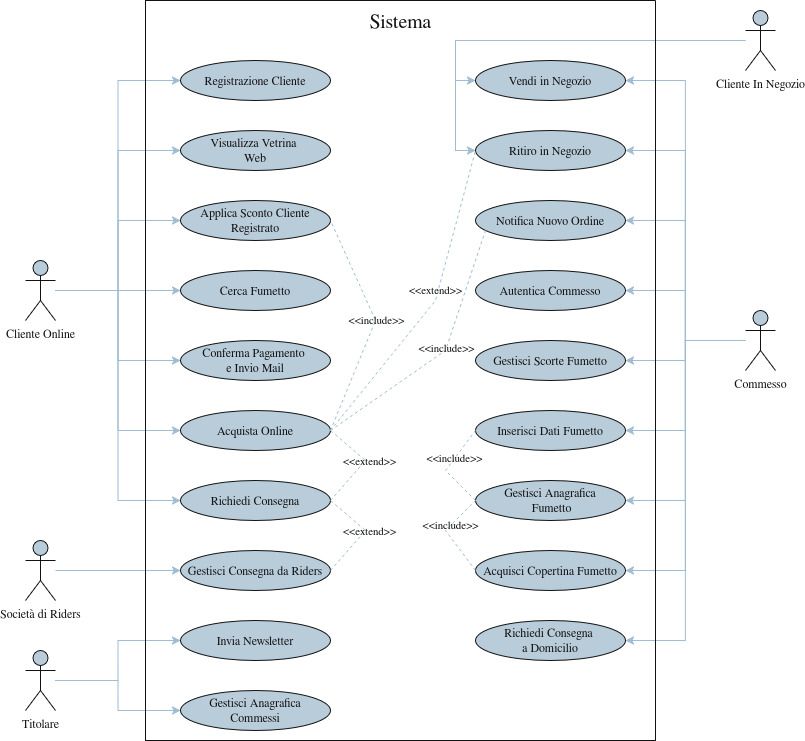
\includegraphics[scale=0.58]{./public/usecasediagram.jpg}
\end{center}

\section{Stima dei Costi}
\subsection{Analisi Function Points}
\subsubsection{Classificazione delle funzioni nelle categorie IFPUG}
Per stimare i costi di sviluppo del sistema utilizziamo il metodo dei Function Points basato sullo standard IFPUG.
\begin{itemize}
  \item \textbf{ILF (Internal Logical Files):}  
    \begin{itemize}
      \item Fumetti
      \item Commessi 
      \item Clienti registrati 
      \item Ordini
    \end{itemize}

  \item \textbf{EIF (External Interface Files):}  
    \begin{itemize}
      \item Sistema di spedizioni (riders): dati di ritiro/consegna e notifiche di avvenuta consegna  
    \end{itemize}

  \item \textbf{EI (External Inputs):}  
    \begin{itemize}
      \item Inserimento nuovo fumetto  
      \item Inserimento nuovo commesso 
      \item Registrazione nuovo cliente 
      \item Inserimento ordine online   
      \item Modifica scorte in negozio
      \item Richiesta consegna a domicilio 
    \end{itemize}

  \item \textbf{EO (External Outputs):}  
    \begin{itemize}
      \item Visualizzazione vetrina web
      \item Invio e-mail di conferma ordine con QR code  
      \item Notifica nuovi ordini ai commessi 
      \item Invio mensile newsletter
    \end{itemize}
  \item \textbf{EQ (External Inquiries):}  
    \begin{itemize}
      \item Ricerca fumetti disponibili
      \item Ricerca ordini attivi
      \item Ricerca consegne in corso
      \item Ricerca fumetti per genere     
      \item Ricerca fumetti per serie 
    \end{itemize}
\end{itemize}
\subsubsection{Calcolo degli UFP}
Di seguito si riporta la tabella standard per l’assegnazione dei pesi IFPUG\begin{center}

\begin{longtable}{|l|c|c|c|}
\hline
\textbf{Categoria} & \textbf{Peso Basso} & \textbf{Peso Medio} & \textbf{Peso Alto} \\
\hline
\endfirsthead

EI (External Inputs)           & 3  & 4  & 6  \\
\hline
EO (External Outputs)          & 4  & 5  & 7  \\
\hline
EQ (External Inquiries)        & 3  & 4  & 6  \\
\hline
ILF (Internal Logical Files)   & 7  & 10 & 15 \\
\hline
EIF (External Interface Files) & 5  & 7  & 10 \\
\hline
\end{longtable}

\end{center}
Procedendo con il calcolo dei UFP si ha:

\begin{longtable}{|
    >{\centering\arraybackslash}p{0.15\textwidth}  % Categoria
    |>{\raggedright\arraybackslash}p{0.50\textwidth} % Funzione
    |>{\centering\arraybackslash}p{0.10\textwidth}  % Peso
    |>{\centering\arraybackslash}p{0.10\textwidth}  % UFP
|}
\hline
\textbf{Categoria} & \textbf{Funzione} & \textbf{Peso} & \textbf{UFP} \\
\hline
\endfirsthead

\hline
\textbf{Categoria} & \textbf{Funzione} & \textbf{Peso} & \textbf{UFP} \\
\hline
\endhead

ILF  
  & Fumetti  & 10 & 10 \\
\hline
ILF  
  & Commessi
  & 10 & 10 \\
\hline
ILF  
  & Clienti registrati  & 10 & 10 \\
\hline
ILF  
  & Ordini  & 10 & 10 \\
\hline
EIF  
  & Sistema di spedizioni (riders): dati di ritiro/consegna e notifiche 
  & 5 & 5 \\
\hline
EI  
  & Inserimento nuovo fumetto  & 6 & 6 \\
\hline
EI  
  & Inserimento nuovo commesso
  & 4 & 4 \\
\hline
EI  
  & Registrazione nuovo cliente
  & 4 & 4 \\
\hline
EI  
  & Inserimento ordine online 
  & 4 & 4 \\
\hline
EI  
  & Modifica scorte in negozio 
  & 4 & 4 \\
\hline
EI  
  & Richiesta consegna a domicilio  & 4 & 4 \\
\hline
EO  
  & Visualizzazione vetrina web   & 7 & 7 \\
\hline
EO  
  & Invio e-mail di conferma ordine con QR code 
  & 4 & 4 \\
\hline
EO  
  & Notifica nuovi ordini ai commessi   & 5 & 5 \\
\hline
EO  
  & Invio mensile newsletter ai clienti registrati 
  & 4 & 4 \\
\hline
EQ  
  & Ricerca fumetti disponibili 
  & 4 & 4 \\
\hline
EQ  
  & Ricerca ordini attivi 
  & 4 & 4 \\
\hline
EQ  
  & Ricerca consegne in corso 
  & 4 & 4 \\
\hline
EQ  
  & Ricerca fumetti per genere 
  & 4 & 4 \\
\hline
EQ  
  & Ricerca fumetti per serie
  & 4 & 4 \\
\hline
\multicolumn{3}{|l|}{\textbf{Totale UFP}} & \textbf{111} \\
\hline
\end{longtable}
\subsubsection{Calcolo del VAF}
Di seguito viene riportata la tabella contentente i fattori correttivi
\begin{longtable}{|
    >{\bfseries}p{0.65\textwidth} 
    |>{\centering\arraybackslash}p{0.25\textwidth}
|}
\hline
\textbf{Caratteristiche generali} & \textbf{Valore} \\
\hline
\endfirsthead

Comunicazione dati & 3 \\
\hline
Distribuzione elaborazione & 0 \\
\hline
Prestazioni & 1 \\
\hline
Utilizzo intensivo configurazione & 0 \\
\hline
Frequenza delle transazioni & 2 \\
\hline
Inserimento dati interattivo & 4 \\
\hline
Efficienza per l’utente finale & 4 \\
\hline
Aggiornamento interattivo & 1 \\
\hline
Complessità elaborativa & 1 \\
\hline
Riusabilità & 1 \\
\hline
Facilità installazione & 0 \\
\hline
Facilità gestione operativa & 2 \\
\hline
Molteplicità di siti & 2 \\
\hline
Facilità di modifica & 2 \\
\hline
\end{longtable}
Il calcolo del Value Adjustment Factor risulta
\[\text{VAF} = 0,65 + 0,01 \times 23 = 0,88\]
\subsubsection{Calcolo degli AFP}
Il calcolo degli Adjusted Function Points risulta
\[\text{AFP}= \text{UFP} \times \text{VAF} = 111\times 0,88 \approx 98 \text{FP}\]
\subsection{Effort e Costo}
Stimiamo i parametri aziendali di \textbf{produttività} e di \textbf{costo orario} come:
\begin{itemize}
  \item \textbf{Produttività}: $8 \text{h/FP}$
  \item \textbf{Costo orario}: $15\text{€/h}$ 
\end{itemize}
Da cui si ricava l'Effort e il costo totale:
\begin{itemize}
  \item \textbf{Effort Totale} = AFP $\times$ Effort = $781,44$h
  \item \textbf{Costo Totale} =  Effort Totale $\times$ Costo = $11721,60$€
\end{itemize}












\end{document}
